\documentclass[conference]{IEEEtran}
\usepackage[utf8]{inputenc}
\usepackage{blindtext, graphicx}
\usepackage{tikz}
\usepackage{tikz}
% we want ER + above/below + left/right
\usetikzlibrary{er,positioning}
\hyphenation{op-tical net-works semi-conduc-tor}

\begin{document}

\title{The usability and buildability of an open source Monitoring Box}

\author{
	\IEEEauthorblockN{Mick Nieman}
	\IEEEauthorblockA{Business IT \& Management\\Amsterdam University\\of Applied Sciences\\
		Wibautstraat 2-4 1091GM Amsterdam\\
		The Netherlands\\
		Mick.Nieman@hva.nl
		}		
	\and
		\IEEEauthorblockN{Pjotr Scholtze}
		\IEEEauthorblockA{Software Engineering \\Amsterdam University\\of Applied Sciences\\
			Wibautstraat 2-4 1091GM Amsterdam\\
			The Netherlands\\
			Pjotr.Scholtze@hva.nl
			}			
		\and
			\IEEEauthorblockN{Heeyeon Joung}
			\IEEEauthorblockA{Electrical Engineering\\Seoul National University\\
			of Science and Technology \\
			Seoul Nowon-gu, Gongneung-dong,\\
			Gongneung-ro 232, South-Korea\\
			Julia.Joung@hva.nl
			}	
		}
	

\maketitle	



\begin{abstract}
This paper is written in commission of the Citizen Data lab from Amsterdam. The main goal of this report is to avoid pitfalls and find solutions for making an open source data-gathering platform. Commissioner of this research is Wouter Meys, Lab Coordinator of the Citizen Data Lab. The reason for this research, along with a developed prototype is the lack of useful environmental data-loggers which also keep track of the GPS-coordinates. This is critical for the Citizen Data Lab when they are, what they call, 'mapping the city'. \\

\end{abstract}

\begin{IEEEkeywords}
Open-source, usability, buildability, environment, data logging
\end{IEEEkeywords}

\IEEEpeerreviewmaketitle

\section{Introduction}
 Researchers nowadays use data to answer the questions asked within their research, that is how research is done. Because of this collecting data for their research is also part of the researchers their task-list and that is not as easy as it seems. Data is collected by researchers doing so called 'data-sprints', this is where a group of people try to collect as much data as possible to do new findings on a certain topic. This is not different for the Citizen Data Lab and their researchers who do research, and back their research, by collecting data through data-sprints. Lately they find their selves struggling collecting the data and most important a specific aspect of their data, the location. For this very reason the development of the Monitoring Box began. The monitoring box tries to hand a solution to the researchers that not only is very convenient but also something researchers can build individually and without any interference of third parties. This way the costs stay low and the usability high. \par
This paper is a result of findings made during the development phase and the testing phase of the prototype of the monitoring box. The paper is written based on the findings and used to be learnt from when further developing the monitoring box. It may also be used by others developing similar open source data gathering platforms.

\subsection{Statement of Purpose}
This has no content yet and needs to be filled in. 

\subsection{Statement of Significance}
This has no content yet and needs to be filled in. 

\section{Research Questions}

\subsection{Overall research question}
What factors contribute to creating an open source, multi-research, sensor geolocation aware, data gathering platform that can be used by the students and researchers from the Makerslab on the Amsterdam University of applied sciences?

\subsection{Sub-questions}
\begin{enumerate}
\item How technical are the students and researchers from the Makerslab on the Amsterdam University of applied sciences?
\begin{enumerate}
\item What documentation is needed and how detailed should it be
\end{enumerate}
\item What improves the usability of the product when taking the structure plane of user experience into account?
\item How can the data be made available such that the students \& researchers from the Minor Makerslab can use it?
\end{enumerate}

\section{Review of literature}
This has no content yet and needs to be filled in. 

\section{Methods}
	To conduct the research a prototype that can be build multiple times is required. Therefore a prototype was created before user studies were preformed. And further modified during the research process. In order to complete the research we carried out the following steps:
	\begin{enumerate}
		\item Identify the use cases of the system.
		\item Generalize the use cases to a generic platform design.
		\item Create prototype.
		\item Research usability concerns.
	\end{enumerate}
	\subsection{Prototype}
		The prototype consists of a base station (a Raspberry Pi) and different sensors (using Arduino's). To make sure that the whole setup stayed modular a translation part (the Arduino's) were used. This design ensures that the base station only needs to know one protocol and does not need to know the individual sensors. ("Designing Multi-Agent Systems around a Programmable Communication Abstraction") Which allows the base station  to focus on using recording the data, managing data storage and making the sensors dynamically attachable.
		\begin{figure}[ht]
			\centering
			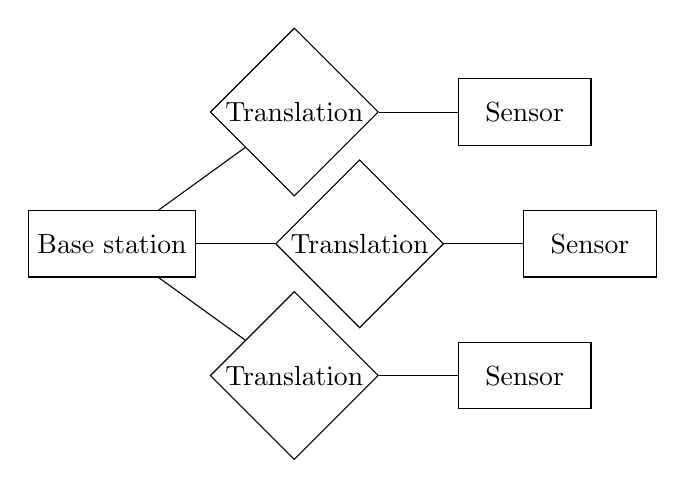
\begin{tikzpicture}[auto,node distance=1cm]
				\node[entity] (node1) {Base station}
								[grow=up,sibling distance=3cm];
				% Now place a relation (ID=rel1)
				\node[relationship] (rel1) [below right = of node1] {Translation};
				\node[relationship] (rel2) [right = of node1] {Translation};
				\node[relationship] (rel3) [above right = of node1] {Translation};
				% Now the 2nd entity (ID=rel2)
				\node[entity] (node2) [right = of rel1]	{Sensor};
				\node[entity] (node3) [right = of rel2]	{Sensor};
				\node[entity] (node4) [right = of rel3]	{Sensor};
				% Draw an edge between rel1 and node1; rel1 and node2
				\path (rel1) edge node {} (node1)
							edge	 node {}	(node2);
				\path (rel2) edge node {} (node1)
							edge	 node {}	(node3);
				\path (rel3) edge node {} (node1)
							edge	 node {}	(node4);
			\end{tikzpicture}
			\caption{Example connection diagram prototype}
		\end{figure}
		\paragraph{Prototype parts}
			\begin{enumerate}
				\item Base station
					\begin{enumerate}
						\item Wifi accesspoint
						\item Web interface
						\item Recording
					\end{enumerate}
				\item Sensors
					\begin{enumerate}
						\item GPS
						\item Temperature and humidity sensor
						\item CO2 sensor (two types)
						\item Heartrate sensor
						\item Galvanic skin response sensor
						\item Camera (PIcam)
					\end{enumerate}
			\end{enumerate}
		\paragraph{Prototype features}
			The base station allows all sensors to be plug and play while on except the Picam. Each sensor can be seen on the web interface or via the screen on the base station. The recordings can only be started via the touchscreen on the base station. Recordings can be downloaded from the web interface or via USB stick that can be mounted on the base station. Every sensor is attached to the base station via USB for ease of use and availability of the devices. An USB hub can easily be used to extend the amount of sensors the base station can handle simultaneously. 
	\subsection{Research}
		In this section is described how each sub question of our main research question is researched. So as to decide the effective method of research we have considered what we needed to do with the research. We considered what should be focused more between breadth and depth or between quantification and qualification and what would be more efficient in empirical research and desk research in each sub question. Along with these considerations, we have came to the following decision. 

		First, to research 'how technical are the students and researchers from the Makerslab on the Amsterdam University of applied sciences?', We let students and researchers from the Makerslab use the Monitoring box. Because we wanted to gain various types of students and researchers in technical point, panels of survey should be breadth. With this we can determine what explanation is needed according to the technical level. So, questions of survey include users' comments so to gain insight in to this. 

		Second, in order to research 'What improves the usability of the product when taking the structure plane of user experience into account?', surveys and desk research are used. And compare this with the shortcomings in usability aspects through existing, similar-functioning platforms and devices. In order to research the Monitoring box in the direction of improving the insufficient aspects of usability.

		Third, in order to research the question 'How can the data be made available such that the students \& researchers from the Minor Makerslab can use it?' desk research is used. We look at other similar cases and consider choosing the most appropriate way of data sharing and how researchers use open source and data gathering platforms.
	\paragraph{Interview setup} The interviews were executed in the following order:
		\begin{enumerate}
			\item Give general introduction to the project to participant.
			\item Let participant assemble hardware and upload software.
			\item During assembly of product observe participant.
			\item Let the participant test their work.
			\item Let participant use the prototype.
			\item Ask participant questions from the survey and ask for general feedback.
		\end{enumerate}
		The interviews were recorded with a camera and notes were made during this interview. Of our team all team members were present, one member controlled the camera, one made notes and one did the presentation.
	\paragraph{Interview participants}
		In order to get an accurate picture of user group, a sample with different backgrounds were chosen. This included students and researchers with different levels of technical skills. The participants of the interviews can be categorized in to the following categories:
		\begin{figure}[ht]
			\centering
			\begin{tabular}{ | l | r | l | }
				\hline
				Type			& Amount	& Description \\ \hline \hline
				Researcher		& 2			& Different technical levels* \\ \hline
				Master-students	& 0			& Did not take part \\ \hline \hline
				Student			& 4			& See figure ... for details \\ \hline \hline
				Total			& 6			& \\ \hline
			\end{tabular}
			\caption{General distribution of participants}
		\end{figure}\\
		The master students were unfortunately unavailable for our research. The student group can be sub divided into different sub-categories:
		\begin{figure}[ht]
			\centering
			\begin{tabular}{ | l | r | l | }
				\hline
				Type					& Amount \\ \hline \hline
				Business IT				& 1 \\ \hline
				Game design				& 1 \\ \hline
				Software engineering	& 2 \\ \hline
				Design					& 1? \\ \hline \hline
				Total					& 4 \\ \hline
			\end{tabular}
			\caption{Major of the participating students}
		\end{figure} \\
		This shows a users from varying backgrounds participated in the research. However unfortunately because of time and resources we had limitation in size of this group
\section{Results}
\begin{enumerate}
\item How technical are the students and researchers from the Makerslab on the Amsterdam University of applied sciences?
\begin{enumerate}
\item What documentation is needed and how detailed should it be
\end{enumerate}
 We wrote 'Manual Monitoring Box' documentation based on the subjective answer to 'What documentation is needed and how detailed should it be'. We started with a list of parts we used and a brief introduction to them. Since we thought there might be some people who are new to the Arduino program, we explain how to install the software, how to upload it to Arduino, and how to get the results. And for each sensor, we describe how the Arduino and the sensor should be connected by schematic and letter. We invited two researchers and three students from the Amsterdam University of applied sciences and require them building the Monitoring box based on our 'Manual Monitoring Box'. \\
As a result, their technical level varied. Each student and researcher had their background knowledge, but they were all different. There is no mention of how to use the breadboard and how to soldering in the manual, but two researchers commented on it. One student pointed out the order of pictures and text. We added the picture of schematics and wrote the explain of schematics after the picture. However, the number in the picture was not clear, which caused a mistake. In fact, one researcher had difficulties in trying to connect only with the picture, and one student also had difficulty connecting, even though he had several experience of Arduino.\\
In conclusion, to create a monitoring box, you need a piece of hardware such as a circuit and a software knowledge such as raspberry pie and arduino. The range of hardware and software is very large and we can not measure and decide someone's technical level through the monitoring box buildability interview. However, depending on their own experience and background knowledge, there may be a first-hand knowledge of re-building this monitoring box. So the documentation for the students and researchers form the Makerslab on the Amsterdam University of applied sciences should be as detailed as possible including the structure of the plate, the principle of circuit connection, the necessary preparations and precautions for soldering.\\
 
\item What improves the usability of the product when taking the structure plane of user experience into account?

In interaction design in the structure plane of user experience, users must communicate correctly to the monitoring box and the monitoring box must deliver the information that the user wants immediately and accurately. In this respect, the Monitoring box has a touch screen and we have added four menus in this screen so that when the user has the information they want, they can instantly check the menu. The home screen shows what percentage of the storage capacity is in use and if users select 'Sensor' menu from the Monitoring Box, users can see the currently connected sensor. And if users select 'Wifi' menu from Monitoring Box, users can confirm the Wifi name and password.//
In information architecture in the structure plane of user experience, it should facilitate intuitive access to data. So we used wireless WiFi so that we could check the information if we had an internet capable device. And with a single push of a button on the Internet Web site, users are able to download the data of the sensors they had recorded at a glance. In addition, the monitoring box screen design allows intuitive use of the menu.


\item How can the data be made available such that the students \& researchers from the Minor Makerslab can use it?

We thought that in order for users to easily access data, they had to be able to see the data at a glance and approach it in an uncomplicated way. So we make the data users have recorded download at once and use the wireless data transmitter to view the data, even if users do not have a certain cable, users can see data only if they have a laptop or smart phone nearby. \\
There are some steps for Makerslab students and researchers to use. The monitoring box is equipped with Wi-Fi function. First, use a computer, laptop or mobile phone to connect to the monitoring box WiFi. And users can access the monitoring box web page by accessing 'monitoring.box:5000' on the web page. In this web page, users can see which sensor is connected now and download recoded data. 
\end{enumerate}

\section{Conclusion}
This has no content yet and needs to be filled in. 

\section{Discussion}
Looking at the main research question you may say that there is a variety of factors that contribute to the successful creation of an open source, multi-research, sensor geolocation aware, data gathering platform that can be used by the students and researchers from the Makerslab on the Amsterdam University of Applied Sciences. The usability is different for every device and modification of a device. Slight alternations may result in a total different user experience and the usability aspects. \\
As there are not much projects similar to this project the main difference shows that this project has no 'custom made' items. Everything can be bought as separate parts from different suppliers. Though this requires some extra work it provides a higher certainty of availability. \\
It could be said that this report and the results of the research only apply to the Monitoring Box. This is partially true, though any researcher or developer well informed about the topic they are going to research for can determine what results may apply to their product and what may not.

\section{Limitations}
This has no content yet and needs to be filled in. 



\bibliography{Research_Report_Monitoring_Box}

\appendices
\section{Baseline of questions asked during user tests}
\begin{enumerate}
\item Which field do you have expertise in?
\item What is your level of technology in hardware?
\item What is your level of technology in software
\item How does the explanation of the parts in the manual help you using the monitoring box?
\item Do you think developers with similar technical levels can make and use the monitoring box as well?\item What could be improved when looking at the monitoring box?
\item What could be improved when looking at the manual?
\end{enumerate}

\end{document}
